% Code Arena — Cara Main & Mekanik (maks. 10 slide)
% Render: tectonic cara-main.tex   (atau: xelatex / pdflatex cara-main.tex)
\documentclass[aspectratio=169,10pt]{beamer}

\usepackage{tikz}
\usetikzlibrary{arrows.meta,positioning,calc,shapes.geometric}
\usepackage{tabularx}
\usepackage{booktabs}
\usepackage{array}

% ---------------------------------------------------------------- warna (sama dengan UI)
\definecolor{navy}{HTML}{0F1724}
\definecolor{ink}{HTML}{1B2537}
\definecolor{cyanx}{HTML}{0E9FB3}
\definecolor{amber}{HTML}{C98A0B}
\definecolor{redx}{HTML}{D83A3A}
\definecolor{purplex}{HTML}{7A5AF0}
\definecolor{greenx}{HTML}{1E9E67}
\definecolor{greyx}{HTML}{6B778A}
\definecolor{paper}{HTML}{F6F8FB}

\setbeamercolor{background canvas}{bg=white}
\setbeamercolor{frametitle}{fg=white,bg=navy}
\setbeamercolor{title}{fg=white}
\setbeamercolor{normal text}{fg=ink}
\setbeamercolor{structure}{fg=cyanx}
\setbeamercolor{itemize item}{fg=cyanx}
\setbeamercolor{itemize subitem}{fg=greyx}
\setbeamercolor{enumerate item}{fg=cyanx}
\setbeamercolor{block title}{fg=white,bg=ink}
\setbeamercolor{block body}{bg=paper}
\setbeamerfont{frametitle}{size=\large,series=\bfseries}
\setbeamertemplate{navigation symbols}{}
\setbeamertemplate{itemize items}[circle]
\setbeamertemplate{enumerate items}[default]
\setbeamertemplate{blocks}[rounded]
\setbeamertemplate{frametitle}{%
  \nointerlineskip
  \begin{beamercolorbox}[wd=\paperwidth,ht=2.5ex,dp=1.2ex,leftskip=1.2em]{frametitle}
    \usebeamerfont{frametitle}\insertframetitle
    \hfill{\normalsize\color{white!70}\textsc{code arena}}\hspace{1.2em}
  \end{beamercolorbox}\vspace{0.4em}}
\setbeamertemplate{footline}{%
  \hfill{\scriptsize\color{greyx}\insertframenumber/\inserttotalframenumber}\hspace{1em}\vspace{0.6em}}
\setlength{\leftmargini}{1.1em}
\setlength{\leftmarginii}{1em}

% badge status (warna + teks, bukan warna saja)
\newcommand{\badge}[2]{\tikz[baseline=(b.base)]\node(b)[draw=#1,fill=#1!10,text=#1!75!black,rounded corners=2pt,inner xsep=2.5pt,inner ysep=1.5pt,font=\scriptsize\sffamily\bfseries]{#2};}
\newcommand{\sbadge}[2]{\tikz[baseline=(b.base)]\node(b)[draw=#1,fill=#1!10,text=#1!75!black,rounded corners=1.5pt,inner xsep=1.6pt,inner ysep=1.1pt,font=\tiny\sffamily\bfseries]{#2};}
\newcommand{\hl}[1]{\textcolor{cyanx}{\textbf{#1}}}
\newcommand{\warn}[1]{\textcolor{redx}{\textbf{#1}}}
\newcolumntype{L}{>{\raggedright\arraybackslash}X}

\begin{document}

% ============================================================== 1. JUDUL
{
\setbeamercolor{background canvas}{bg=navy}
\begin{frame}[plain]
  \begin{tikzpicture}[remember picture,overlay]
    \node[anchor=north west,text=white,font=\Huge\bfseries] at ([xshift=2.2em,yshift=-4.2em]current page.north west) {CODE ARENA};
    \node[anchor=north west,text=cyanx!70,font=\large\ttfamily] at ([xshift=2.3em,yshift=-7.2em]current page.north west) {find the flaw. prove the bug. defend your code.};
    \node[anchor=north west,text=white,font=\Large] at ([xshift=2.3em,yshift=-10.4em]current page.north west) {Cara Main \& Mekanik Permainan};
    \node[anchor=north west,text=white!75,text width=0.62\paperwidth,font=\normalsize] at ([xshift=2.3em,yshift=-13.2em]current page.north west)
      {Recap praktikum Pemrograman Berorientasi Objek (Python) dalam format kompetisi \textbf{attack \& defense} antar kelompok.};
    % ikon ring kecil
    \begin{scope}[shift={([xshift=-8.5em,yshift=-1.2em]current page.east)}]
      \foreach \i/\c in {0/cyanx,1/amber,2/redx,3/purplex,4/greenx}{
        \node[draw=\c,line width=1.4pt,rounded corners=3pt,minimum width=2.6em,minimum height=1.6em,fill=navy] (n\i) at ({90-72*\i}:4.2em) {};}
      \foreach \i/\j in {0/1,1/2,2/3,3/4,4/0}{
        \draw[-{Latex[length=2.2mm]},redx!80,line width=1pt] (n\i) to[bend left=18] (n\j);}
    \end{scope}
    \node[anchor=south west,text=white!55,font=\scriptsize] at ([xshift=2.3em,yshift=1.8em]current page.south west)
      {Mahasiswa: \texttt{/}\quad Instruktur: \texttt{/admin}\quad Proyektor: \texttt{/arena}};
  \end{tikzpicture}
\end{frame}
}

% ============================================================== 2. GAMBARAN BESAR
\begin{frame}{Gambaran besar: apa yang terjadi di Code Arena?}
\begin{columns}[T,onlytextwidth]
\column{0.53\textwidth}
\begin{itemize}\setlength\itemsep{0.35em}
  \item Kelas dibagi menjadi \hl{kelompok}. Setiap ronde memakai satu \hl{challenge} PBO: kode Python yang \warn{sengaja berisi bug} (mis.\ class attribute bersama, name mangling, decorator salah).
  \item Dalam satu ronde setiap tim punya \textbf{dua pekerjaan sekaligus}:
  \begin{itemize}
    \item \textcolor{redx}{\textbf{ATTACK}} --- mencari \& membuktikan bug pada kode tim target.
    \item \textcolor{cyanx}{\textbf{DEFENSE}} --- menutup bug pada kode sendiri dengan patch + regression test.
  \end{itemize}
  \item \hl{Instruktur} menjadi juri: memvalidasi laporan, menilai patch dengan rubric, dan mengesahkan skor.
  \item Semua status, waktu, dan skor ditentukan \textbf{server}; Live Arena menampilkannya secara real-time.
\end{itemize}
\column{0.44\textwidth}
\begin{block}{Alur satu sesi}
\begin{enumerate}\setlength\itemsep{0.15em}\small
  \item Mahasiswa \textbf{join} dengan NIM $\rightarrow$ waiting room.
  \item Instruktur membentuk \textbf{kelompok} (random/manual).
  \item Instruktur membuat \textbf{ronde}: pilih challenge, pairing, durasi.
  \item Ronde berjalan melalui \textbf{6 fase} (slide 5).
  \item Skor ronde disahkan, \textbf{pembahasan} dibuka.
  \item Ulangi ronde dengan challenge lain; \textbf{leaderboard} kumulatif.
\end{enumerate}
\end{block}
\vspace{0.3em}
{\footnotesize\color{greyx} 13 challenge: 12 materi (class \& object, encapsulation, class/static method \& decorator, inheritance, abstract/dataclass/duck typing) + 1 capstone \emph{e-wallet}.}
\end{columns}
\end{frame}

% ============================================================== 3. JOIN & KELOMPOK
\begin{frame}{Langkah 1 --- Join dan pembentukan kelompok}
\begin{columns}[T,onlytextwidth]
\column{0.48\textwidth}
\textbf{Join dengan NIM}
\begin{itemize}\setlength\itemsep{0.2em}\small
  \item Buka alamat Code Arena, ketik \hl{NIM}. NIM dicocokkan dengan roster; NIM tak dikenal ditolak.
  \item NIM \emph{bukan password} --- hanya identitas. \warn{Satu NIM = satu perangkat aktif.} Pindah perangkat? Minta instruktur ``lepas perangkat''.
  \item Koneksi terputus? Buka lagi: identitas dan kelompok \textbf{dipulihkan otomatis}.
\end{itemize}
\textbf{Waiting room}
\begin{itemize}\small
  \item Menampilkan jumlah hadir, siapa yang online, dan status pembentukan kelompok. Halaman berubah sendiri saat kelompok Anda dikonfirmasi.
\end{itemize}
\column{0.49\textwidth}
\textbf{Pembentukan kelompok (instruktur)}
\begin{itemize}\setlength\itemsep{0.2em}\small
  \item \hl{Random}: server mengambil \emph{snapshot} peserta yang menunggu, mengacak, membagi \textbf{seimbang} (selisih maks.\ 1, target 4 orang).
  \item \hl{Manual}: buat/namai kelompok, tambah/pindah anggota.
  \item Hasil berupa \textbf{preview} --- baru terlihat mahasiswa setelah \textbf{dikonfirmasi}.
  \item Datang terlambat $\rightarrow$ tetap menunggu sampai ditempatkan instruktur.
  \item Saat ronde pertama dimulai kelompok \warn{dikunci}; perubahan hanya oleh instruktur dengan alasan tercatat.
\end{itemize}
\vspace{0.3em}
{\footnotesize\color{greyx}Contoh pembagian: 9 hadir $\rightarrow$ 3+3+3 \;$\cdot$\; 13 $\rightarrow$ 4+3+3+3 \;$\cdot$\; 18 $\rightarrow$ 4+4+4+3+3 \;$\cdot$\; 20 $\rightarrow$ 5 kelompok @4.}
\end{columns}
\end{frame}

% ============================================================== 4. PAIRING
\begin{frame}{Langkah 2 --- Pairing: siapa menyerang siapa?}
\begin{columns}[c,onlytextwidth]
\column{0.42\textwidth}
\centering
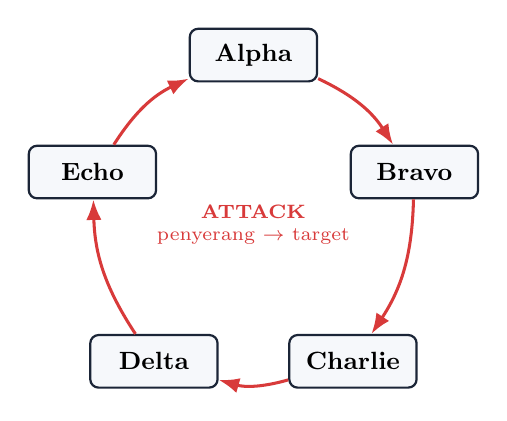
\begin{tikzpicture}[team/.style={draw=ink,fill=paper,rounded corners=3pt,minimum width=4.6em,minimum height=1.9em,font=\small\bfseries,line width=0.8pt}]
  \foreach \i/\n in {0/Alpha,1/Bravo,2/Charlie,3/Delta,4/Echo}{
    \node[team] (t\i) at ({90-72*\i}:2.15cm) {\n};}
  \foreach \i/\j in {0/1,1/2,2/3,3/4,4/0}{
    \draw[-{Latex[length=2.6mm]},redx,line width=1.1pt] (t\i) to[bend left=16] (t\j);}
  \node[font=\scriptsize,text=redx,align=center] at (0,0) {\textbf{ATTACK}\\penyerang $\rightarrow$ target};
\end{tikzpicture}
\column{0.56\textwidth}
\begin{itemize}\setlength\itemsep{0.35em}
  \item Setiap tim \textbf{menyerang tepat satu} tim dan \textbf{diserang tepat satu} tim --- tidak ada yang menganggur, tidak ada yang dikeroyok.
  \item Semua tim mengerjakan \hl{challenge yang sama} dan mulai dari \hl{starter code yang sama}.
  \item Pairing dibuat server (acak, menghindari saling-serang dua arah dan pengulangan pasangan ronde sebelumnya). Instruktur boleh mengubahnya sebelum ronde dimulai.
  \item Saat ronde dimulai pairing \warn{dikunci}: tidak berubah karena refresh, reconnect, atau aksi siapa pun.
\end{itemize}
\vspace{0.3em}
{\footnotesize
\begin{tabular}{@{}lll@{}}\toprule
Tim & Menyerang $\rightarrow$ & Diserang oleh $\leftarrow$\\\midrule
Alpha & Bravo & Echo\\ Bravo & Charlie & Alpha\\ \dots & \dots & \dots\\\bottomrule
\end{tabular}}
\end{columns}
\end{frame}

% ============================================================== 5. FASE
\begin{frame}{Langkah 3 --- Enam fase dalam satu ronde}
\footnotesize
\renewcommand{\arraystretch}{1.25}
\begin{tabularx}{\textwidth}{@{}>{\raggedright\arraybackslash\bfseries}p{0.17\textwidth}LL>{\raggedright\arraybackslash}p{0.14\textwidth}@{}}
\toprule
Fase & Yang terjadi & Yang dikerjakan tim & Ditutup oleh\\\midrule
1. Briefing & Challenge \& rubric diumumkan. & Baca spesifikasi \& starter code. & Instruktur\\
2. Defense Prep & Editor pertahanan dibuka. & Perbaiki bug yang Anda temukan sendiri, lalu \textbf{SIMPAN} draft. & Timer / instruktur\\
3. \textcolor{redx}{Attack Window} & Server \textbf{mengunci snapshot v1} setiap tim. & \textcolor{redx}{Attack}: uji snapshot target, kirim laporan. \textcolor{cyanx}{Defense}: pantau laporan masuk, mulai patch. & Timer / instruktur\\
4. Defense Response & Laporan \textbf{dikunci} (tidak bisa dikirim lagi). & Selesaikan \& submit patch + regression test, ajukan rebuttal. & Timer / instruktur\\
5. Verification & Instruktur memvalidasi laporan \& patch. & Menunggu hasil; baca feedback review. & Instruktur\\
6. Round Results & Skor dihitung lalu \textbf{disahkan}. & Lihat leaderboard; pembahasan \& answer key dibuka. & Instruktur\\\bottomrule
\end{tabularx}
\vspace{0.6em}
\begin{itemize}\setlength\itemsep{0.15em}
  \item \hl{Waktu milik server}: countdown sama di semua layar; refresh tidak mengulang timer. Saat waktu habis server menutup fase otomatis.
  \item Aksi setelah deadline \warn{ditolak}. Saat instruktur \textbf{pause}, timer membeku dan semua aksi ditahan.
\end{itemize}
\end{frame}

% ============================================================== 6. SNAPSHOT
\begin{frame}{Mekanik inti --- Locked snapshot (keadilan serangan)}
\centering
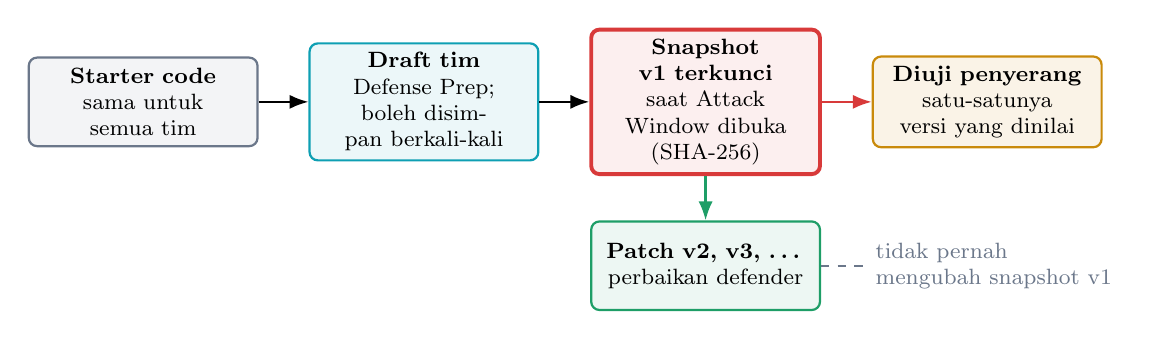
\begin{tikzpicture}[box/.style={draw,rounded corners=3pt,align=center,font=\footnotesize,minimum height=3.2em,text width=7.6em,line width=0.8pt},
  >={Latex[length=2.4mm]}]
  \node[box,draw=greyx,fill=greyx!8] (s) {\textbf{Starter code}\\sama untuk semua tim};
  \node[box,draw=cyanx,fill=cyanx!8,right=1.8em of s] (d) {\textbf{Draft tim}\\Defense Prep; boleh disimpan berkali-kali};
  \node[box,draw=redx,fill=redx!8,right=1.8em of d,line width=1.4pt] (v1) {\textbf{Snapshot v1 terkunci}\\saat Attack Window dibuka (SHA-256)};
  \node[box,draw=amber,fill=amber!10,right=1.8em of v1] (a) {\textbf{Diuji penyerang}\\satu-satunya versi yang dinilai};
  \node[box,draw=greenx,fill=greenx!8,below=1.6em of v1] (p) {\textbf{Patch v2, v3, \dots}\\perbaikan defender};
  \draw[->,thick] (s) -- (d);
  \draw[->,thick] (d) -- (v1);
  \draw[->,thick,redx] (v1) -- (a);
  \draw[->,thick,greenx] (v1) -- (p);
  \draw[dashed,greyx,thick] (p.east) -- ++(1.6em,0) node[right,font=\footnotesize,text=greyx,align=left]{tidak pernah\\mengubah snapshot v1};
\end{tikzpicture}
\vspace{0.6em}
\begin{columns}[T,onlytextwidth]
\column{0.49\textwidth}
\begin{itemize}\setlength\itemsep{0.2em}\small
  \item Snapshot = \textbf{versi terakhir yang disimpan} saat Defense Prep. Tidak menyimpan apa pun $\rightarrow$ starter code (beserta semua bug-nya) yang dikunci.
  \item Penyerang hanya bisa melihat snapshot \textbf{target resminya} --- bukan kode tim lain.
\end{itemize}
\column{0.49\textwidth}
\begin{itemize}\setlength\itemsep{0.2em}\small
  \item Defender boleh langsung memperbaiki kodenya, tetapi serangan \warn{tetap dinilai terhadap snapshot v1}. Memperbaiki diam-diam tidak membatalkan temuan lawan.
  \item Artinya: \hl{Defense Prep yang serius = lebih sedikit bug yang bisa diserang.}
\end{itemize}
\end{columns}
\end{frame}

% ============================================================== 7. ATTACK
\begin{frame}{Cara menyerang --- Attack report}
\begin{columns}[T,onlytextwidth]
\column{0.5\textwidth}
\textbf{Alur}
\begin{enumerate}\setlength\itemsep{0.15em}\small
  \item Klik \badge{amber}{MULAI INSPEKSI TARGET}, baca snapshot target, uji kodenya secara lokal (simpan sebagai \texttt{solution.py}).
  \item Temukan perilaku yang \textbf{melanggar spesifikasi}, buat input pemicu \& test case.
  \item Isi laporan $\rightarrow$ \textbf{Simpan draft} $\rightarrow$ \textbf{Submit} (ada konfirmasi).
  \item Laporan terkirim langsung muncul di layar tim target; status Anda \badge{purplex}{MENUNGGU VALIDASI}.
\end{enumerate}
\textbf{Isi laporan}: judul, lokasi kode, input/pemicu, expected vs actual, langkah reproduksi, \hl{root cause}, \hl{konsep PBO}, bukti/test.
\column{0.48\textwidth}
\textbf{Aturan}
\begin{itemize}\setlength\itemsep{0.15em}\small
  \item Setelah submit laporan \warn{terkunci} dan tidak bisa dihapus.
  \item Maks.\ \textbf{6 laporan resmi} per ronde; laporan identik ditolak.
  \item Mengirim laporan \textbf{tidak} otomatis memberi poin.
\end{itemize}
\textbf{Verdict instruktur}\\[0.2em]
{\footnotesize
\begin{tabular}{@{}lp{0.6\linewidth}@{}}
\badge{greenx}{VALID} & Bug terbukti $\rightarrow$ dinilai rubric (maks.\ 25).\\
\badge{redx}{INVALID} & Tidak terbukti $\rightarrow$ 0 poin.\\
\badge{redx}{DUPLICATE} & Sama dengan laporan sebelumnya $\rightarrow$ 0 poin.\\
\badge{amber}{NEEDS REVISION} & Perbaiki \& kirim ulang (riwayat revisi tetap tercatat).\\
\end{tabular}}
\end{columns}
\end{frame}

% ============================================================== 8. DEFENSE
\begin{frame}{Cara bertahan --- Analisis, patch, regression test, rebuttal}
\begin{columns}[T,onlytextwidth]
\column{0.5\textwidth}
\textbf{Incoming reports}
\begin{itemize}\setlength\itemsep{0.15em}\small
  \item Laporan dari penyerang muncul \textbf{real-time} di tab Defense, lengkap dengan isinya.
  \item Tiap laporan punya progres sendiri: \badge{cyanx}{DIANALISIS} \badge{amber}{DIPERBAIKI} \badge{cyanx}{MENULIS TEST} --- tim bisa memperbaiki bug A sambil menunggu review bug B.
\end{itemize}
\textbf{Rebuttal}
\begin{itemize}\small
  \item Yakin laporan salah? Kirim \textbf{rebuttal} dengan alasan teknis (min.\ 20 karakter) \emph{sebelum} laporan direview. Jika instruktur setuju laporan invalid $\rightarrow$ \hl{bonus hingga +10}.
\end{itemize}
\column{0.48\textwidth}
\textbf{Patch}
\begin{itemize}\setlength\itemsep{0.15em}\small
  \item Isi: \textbf{kode lengkap modul} versi perbaikan, \hl{root cause analysis}, \hl{regression test} (\texttt{unittest}, minimal satu \texttt{def test\_...}), penjelasan perilaku normal \& edge case, dan laporan mana yang ditangani.
  \item \textbf{Simpan draft} sesering mungkin $\rightarrow$ \textbf{Submit} untuk review (maks.\ 5 kali per ronde). Patch yang disubmit \warn{dibekukan}; perubahan berikutnya menjadi versi baru.
  \item Versi bersifat \textbf{kumulatif} (v3 berisi perbaikan v2 + yang baru).
  \item Server \textbf{tidak menjalankan} kode Anda: instruktur menilai patch \& test sesuai rubric. Uji sendiri secara lokal sebelum submit!
\end{itemize}
\end{columns}
\end{frame}

% ============================================================== 9. STATUS & ARENA
\begin{frame}{Status tim dan Live Arena}
\noindent{\small Setiap tim punya \textbf{dua status terpisah} yang \warn{hanya berubah karena tindakan nyata} (simpan, submit, review, tombol status) --- bukan karena membuka halaman.}\par\vspace{0.5em}
\begin{columns}[T,onlytextwidth]
\column{0.49\textwidth}
{\scriptsize
\renewcommand{\arraystretch}{1.12}
\begin{tabularx}{\linewidth}{@{}lL@{}}
\textbf{ATTACK} (penyerang) & \textbf{pemicu}\\\midrule
\sbadge{greyx}{TARGET ASSIGNED} & pairing dikunci\\
\sbadge{amber}{INSPECTING TARGET} & tombol tim\\
\sbadge{amber}{PREPARING REPORT} & draft laporan disimpan\\
\sbadge{redx}{REPORT SUBMITTED} & laporan dikirim\\
\sbadge{purplex}{AWAITING VALIDATION} & attack window ditutup\\
\sbadge{greenx}{VALID} \sbadge{redx}{INVALID} \sbadge{redx}{DUPLICATE} & review instruktur\\
\sbadge{greyx}{ATTACK COMPLETED} & ronde disahkan\\
\end{tabularx}}
\column{0.49\textwidth}
{\scriptsize
\renewcommand{\arraystretch}{1.12}
\begin{tabularx}{\linewidth}{@{}lL@{}}
\textbf{DEFENSE} (defender) & \textbf{pemicu}\\\midrule
\sbadge{cyanx}{DEFENSE PREPARATION} & fase dibuka\\
\sbadge{greyx}{AWAITING ATTACK} & snapshot dikunci\\
\sbadge{redx}{ATTACK RECEIVED} & laporan masuk\\
\sbadge{cyanx}{ANALYZING BUG} & analisis disimpan\\
\sbadge{amber}{FIXING BUG} & kode patch disimpan\\
\sbadge{cyanx}{WRITING REGRESSION TEST} & test disimpan\\
\sbadge{purplex}{PATCH SUBMITTED / AWAITING REVIEW} & patch dikirim\\
\sbadge{greenx}{PATCH ACCEPTED} \sbadge{redx}{PATCH REJECTED} & review instruktur\\
\end{tabularx}}
\end{columns}
\vspace{0.6em}
\begin{block}{Live Arena (layar proyektor, \texttt{/arena})}
\footnotesize
\hl{Network view}: kotak = tim, panah \textcolor{redx}{\textbf{ATTACK}} = pairing resmi + jumlah laporan/pending/valid. \;
\hl{Team board}: kartu ATTACK, DEFENSE, dan skor terpisah. \;
Timeline fase, countdown, leaderboard, feed; klik tim/panah untuk detail. \;
Warna: \textcolor{amber}{amber} investigasi, \textcolor{redx}{merah} serangan, \textcolor{cyanx}{cyan} analisis, \textcolor{purplex}{ungu} review, \textcolor{greenx}{hijau} berhasil, \textcolor{greyx}{abu} menunggu --- selalu dengan ikon \& teks. Isi laporan tim lain tidak ditampilkan di arena publik.
\end{block}
\end{frame}

% ============================================================== 10. SKOR
\begin{frame}{Skor, finalisasi, dan tips menang}
\begin{columns}[T,onlytextwidth]
\column{0.55\textwidth}
{\footnotesize
\renewcommand{\arraystretch}{1.15}
\begin{tabularx}{\linewidth}{@{}Lr@{}}\toprule
\textcolor{redx}{\textbf{Attack}} --- per temuan \textbf{valid} & \\
\quad Bug dapat direproduksi & 10\\
\quad Root cause \& konsep PBO akurat & 10\\
\quad Bukti \& test case jelas & 5\\
\quad \textit{2 temuan terbaik per ronde} & \textbf{maks.\ 50}\\\midrule
\textcolor{cyanx}{\textbf{Defense}} --- patch \textbf{terbaik} yang direview & \\
\quad Patch memperbaiki root cause & 20\\
\quad Regression test & 15\\
\quad Perilaku normal \& edge case & 10\\
\quad Penjelasan teknis & 5 \;\textbf{(maks.\ 50)}\\\midrule
\textcolor{purplex}{\textbf{Rebuttal}} benar & \textbf{maks.\ 10}\\\bottomrule
\end{tabularx}}
\\[0.3em]{\scriptsize\textbf{Contoh:} 3 temuan valid bernilai 25, 20, 15 $\rightarrow$ attack = 45. Patch v2 = 38, v3 = 46 $\rightarrow$ defense = 46. Rebuttal +5. \textbf{Total ronde = 96.}}
\column{0.42\textwidth}
\textbf{Finalisasi}
\begin{itemize}\setlength\itemsep{0.1em}\footnotesize
  \item Skor live dihitung ulang dari hasil review; refresh/reconnect tidak menggandakan poin.
  \item Setelah ronde \textbf{disahkan}, skor \warn{terkunci}; perubahan hanya lewat koreksi beralasan yang tercatat.
  \item Leaderboard = jumlah semua ronde.
\end{itemize}
\textbf{Tips menang}
\begin{itemize}\setlength\itemsep{0.1em}\footnotesize
  \item Manfaatkan \textbf{Defense Prep} --- dan \textbf{SIMPAN}.
  \item Laporan \hl{berkualitas} $>$ banyak laporan: root cause \& konsep PBO tepat, sertakan test.
  \item Regression test harus \textbf{gagal di kode lama}, lulus di patch.
  \item Bagi peran attacker/defender; koordinasi lewat \textbf{chat tim}.
\end{itemize}
\end{columns}
\end{frame}

\end{document}
